\documentclass[12pt,letterpaper]{exam}
\usepackage[lmargin=1in,rmargin=1in,tmargin=1in,bmargin=1in]{geometry}
\usepackage{exams}

% Exam Class Documentation: https://ctan.org/pkg/exam?lang=en 
% Compile at least twice, always.

% -------------------
% Course & Exam Information
% -------------------
\newcommand{\course}{Math 999: Exam 1}
\newcommand{\term}{Semester -- Year}
\newcommand{\examdate}{MM/DD/YYYY}
\newcommand{\timelimit}{00 Minutes}


% -------------------
% Content
% -------------------
\begin{document}

\examtitle
\instructions{Write your name on the appropriate line on the exam cover sheet. This exam contains \numpages\ pages (including this cover page) and \numquestions\ questions. Check that you have every page of the exam. Answer the questions in the spaces provided on the question sheets. Be sure to answer every part of each question and show all your work. If you run out of room for an answer, continue on the back of the page --- being sure to indicate the problem number.} 
\scores
\bottomline
\newpage


% ---------
% Questions
% ---------
\begin{questions}


% Question 1
\question[5] Solve the Riemann Hypothesis. Be sure to justify each step.


% Question 2
\newpage
\question Answer the following parts completely. \vspace{0.5cm}
	\begin{parts}
	\part[1] What is Mathematics? \vspace{2cm}
	\part[2] Why are we here? \vfill
	\part[3] What is the meaning of life? \vfill
	\end{parts}


% Question 3
\newpage
\question[1] Write an answer to an unasked question in the space below.
\makeemptybox{2in}


% Question 4
\newpage
\question[3] Write an award winning level novel in the space below. 
\makeemptybox{\fill}


% Question 5
\newpage
\question[1] Choose an option.
	\begin{choices}
	\choice Here is an option.
	\choice Here is another.
	\choice A third choice!
	\end{choices}


% Question 6
\vspace{3cm}
\question[1] Choose an option. \pspace
	\begin{oneparchoices}
	\choice Here is a choice.
	\choice Another choice
	\choice It keeps going!
	\end{oneparchoices}


% Question 7
\vspace{3cm}
\question[1] Mark circle if true.
	\begin{checkboxes}
	\choice This choice is correct.
	\choice The other choice is incorrect. 
	\end{checkboxes}


% Question 8
\vspace{3cm}
{
\checkboxchar{$\Box$}
\question[3] Mark box if true.
	\begin{checkboxes}
	\choice This choice is not true.
	\choice This choice is not false. 
	\end{checkboxes}
}


% Question 9
\newpage
\question[1] Write me something beautiful! 
\fillwithlines{\fill}


% Question 10
\newpage
\question[1] In the space provided, write your autobiography. 
\fillwithdottedlines{27em}


% Question 11
\newpage
{%
	% Defines choice options: \roman, \arabic, etc
%	\renewcommand*\thechoice{\roman{choice}}
%	\renewcommand*\choicelabel{\thechoice)}
\question[1] What is $2+2=$ ?
	\begin{multicols}{2}
	\begin{choices}
	\choice Martha Washington
	\choice Mars
	\choice 17
	\choice 4
	\choice $-4$
	\choice Cannot be determined.
	\choice None of the above.
	\choice All of the above.
	\end{choices}
	\end{multicols}
}%


% Question 12
\newpage
\question[10] Mark the following statements True or False: \pspace
\def\arraystretch{1.5} % increase vertical spacing
\noindent\begin{tabularx}{\textwidth}{cXcc}
 & & True & False \\
(\thepart) & This statement is true. & \boxed{\phantom{\cmark}} & \boxed{\phantom{\cmark}} \\ 

(\thepart) & This statement is false. & \boxed{\phantom{\cmark}} & \boxed{\phantom{\cmark}} \\[3cm]

(\thepart) & The statement above is true. & \boxed{\phantom{\cmark}} & \boxed{\phantom{\cmark}} \\

(\thepart) & The answer to this question is false. & \boxed{\phantom{\cmark}} & \boxed{\phantom{\cmark}}
\end{tabularx}


% Question 13
\newpage
\question Draw a graph below. 
	\[
	\begin{tikzpicture}
	\tkzInit[xmax=7,ymax=7,xmin= -7,ymin= -7]
   	\tkzGrid
   	\tkzAxeXY
  	\end{tikzpicture}
	\]


% Question 14
\newpage
\question Draw a graph below.
	\[
	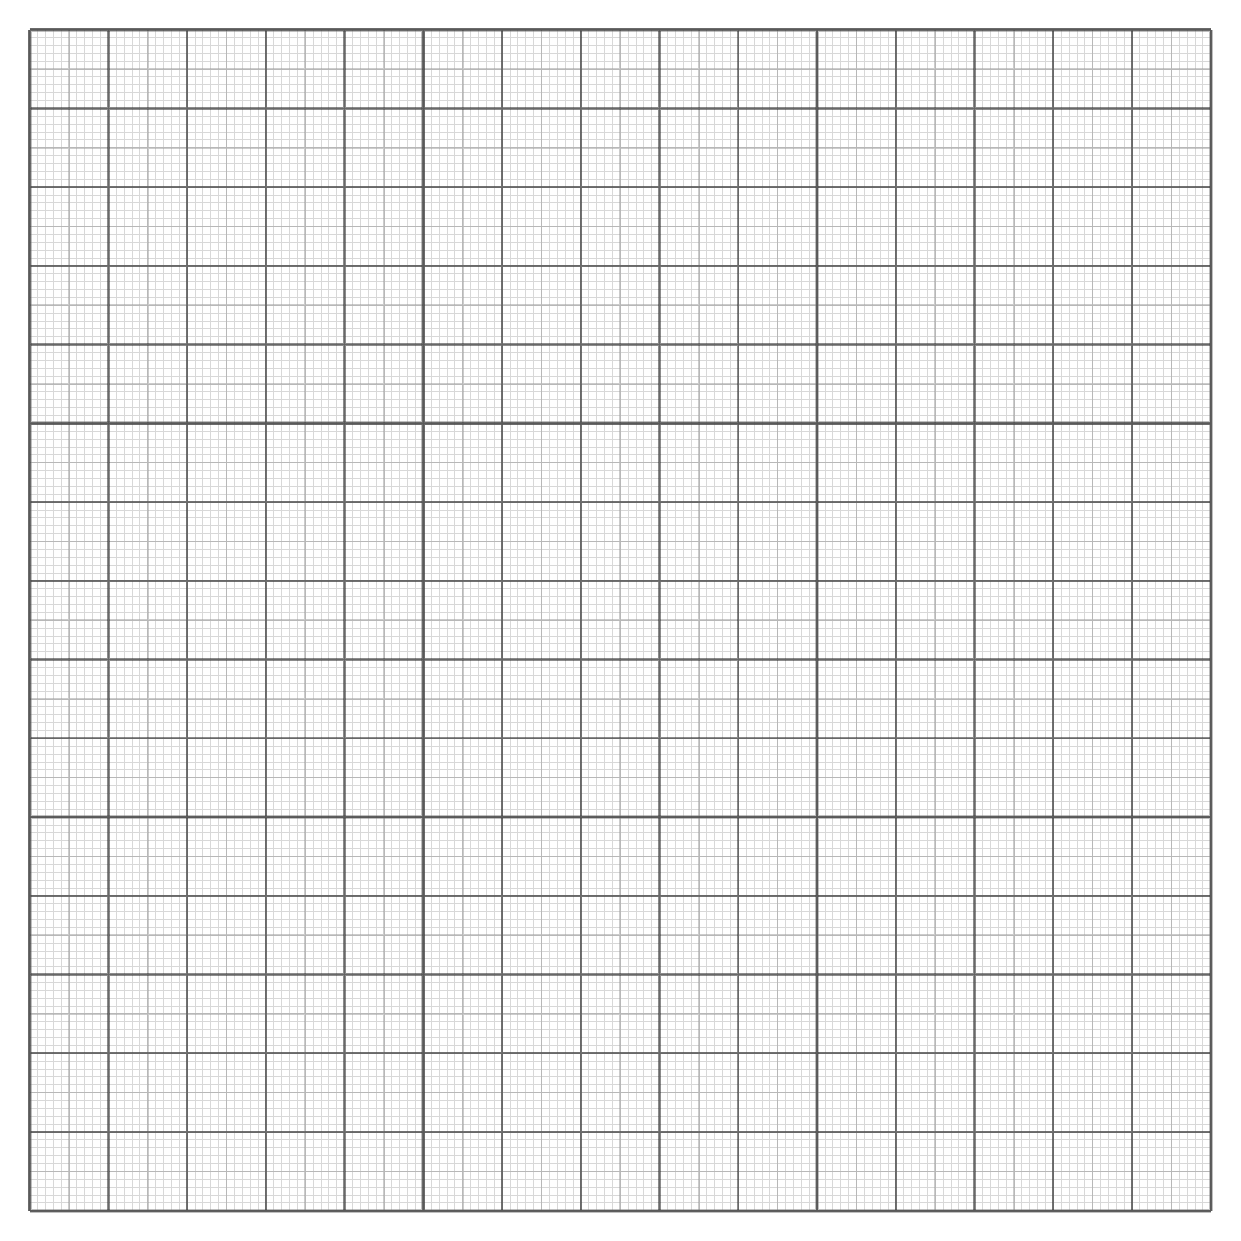
\begin{tikzpicture}[x=1cm, y=1cm, semitransparent]
	\draw[step=1mm, line width=0.1mm, black!30!white] (0,0) grid (15,15);
	\draw[step=5mm, line width=0.2mm, black!40!white] (0,0) grid (15,15);
	\draw[step=5cm, line width=0.5mm, black!50!white] (0,0) grid (15,15);
	\draw[step=1cm, line width=0.3mm, black!90!white] (0,0) grid (15,15);
	\end{tikzpicture}
	\]


\end{questions}
\end{document}